
\documentclass[12pt]{report}
\usepackage{geometry}
\geometry{a4paper}
\usepackage{chicago}
\usepackage{makeidx}
\usepackage{tabularx}
\usepackage{graphicx}
\usepackage{color}
\usepackage{pdfpages}

\def\keywords{\vspace{.5em}
{\textbf{Keywords} \linebreak \,\relax%
}}
\def\endkeywords{\par}


\begin{document}
\begin{titlepage}
\begin{center}

% Upper part of the page. The '~' is needed because \\
% only works if a paragraph has started.
\textbf{\LARGE The University of Birmingham}\\[0.35cm]
\textbf{\LARGE School of Computer Science}\\[0.35cm]
\textbf{\LARGE MSc in Advanced Computer Science}\\[2.5cm]

\textsc{\Large Second semester mini-project}\\[2.5cm]

% Title

{ \huge \bfseries  Analysing User Interaction On Mobile Devices \\[1cm] }

{\large \textbf{Karthikeya Udupa Kuppar Manjunath}\\[1cm]}

\large{Supervisor: Mirco Musolesi}
% Author and supervisor


\vfill

% Bottom of the page
{\large April 2014}

\end{center}
\end{titlepage}

\begin{abstract}

abstract here.
\linebreak\linebreak\linebreak\linebreak
\begin{center}
\begin{keywords}
keywords here.
\end{keywords}
\end{center}
\end{abstract}


\tableofcontents
\listoffigures
\listoftables
\newpage

\chapter{Introduction}
\noindent

\noindent

\section{section 1}
section 1.
\bibliographystyle{ abbrv}
\bibliography{mini_project_report}

%APPENDICES
\appendix
%Mini-project declaration
%\clearpage
\chapter{Mini-Project Declaration}
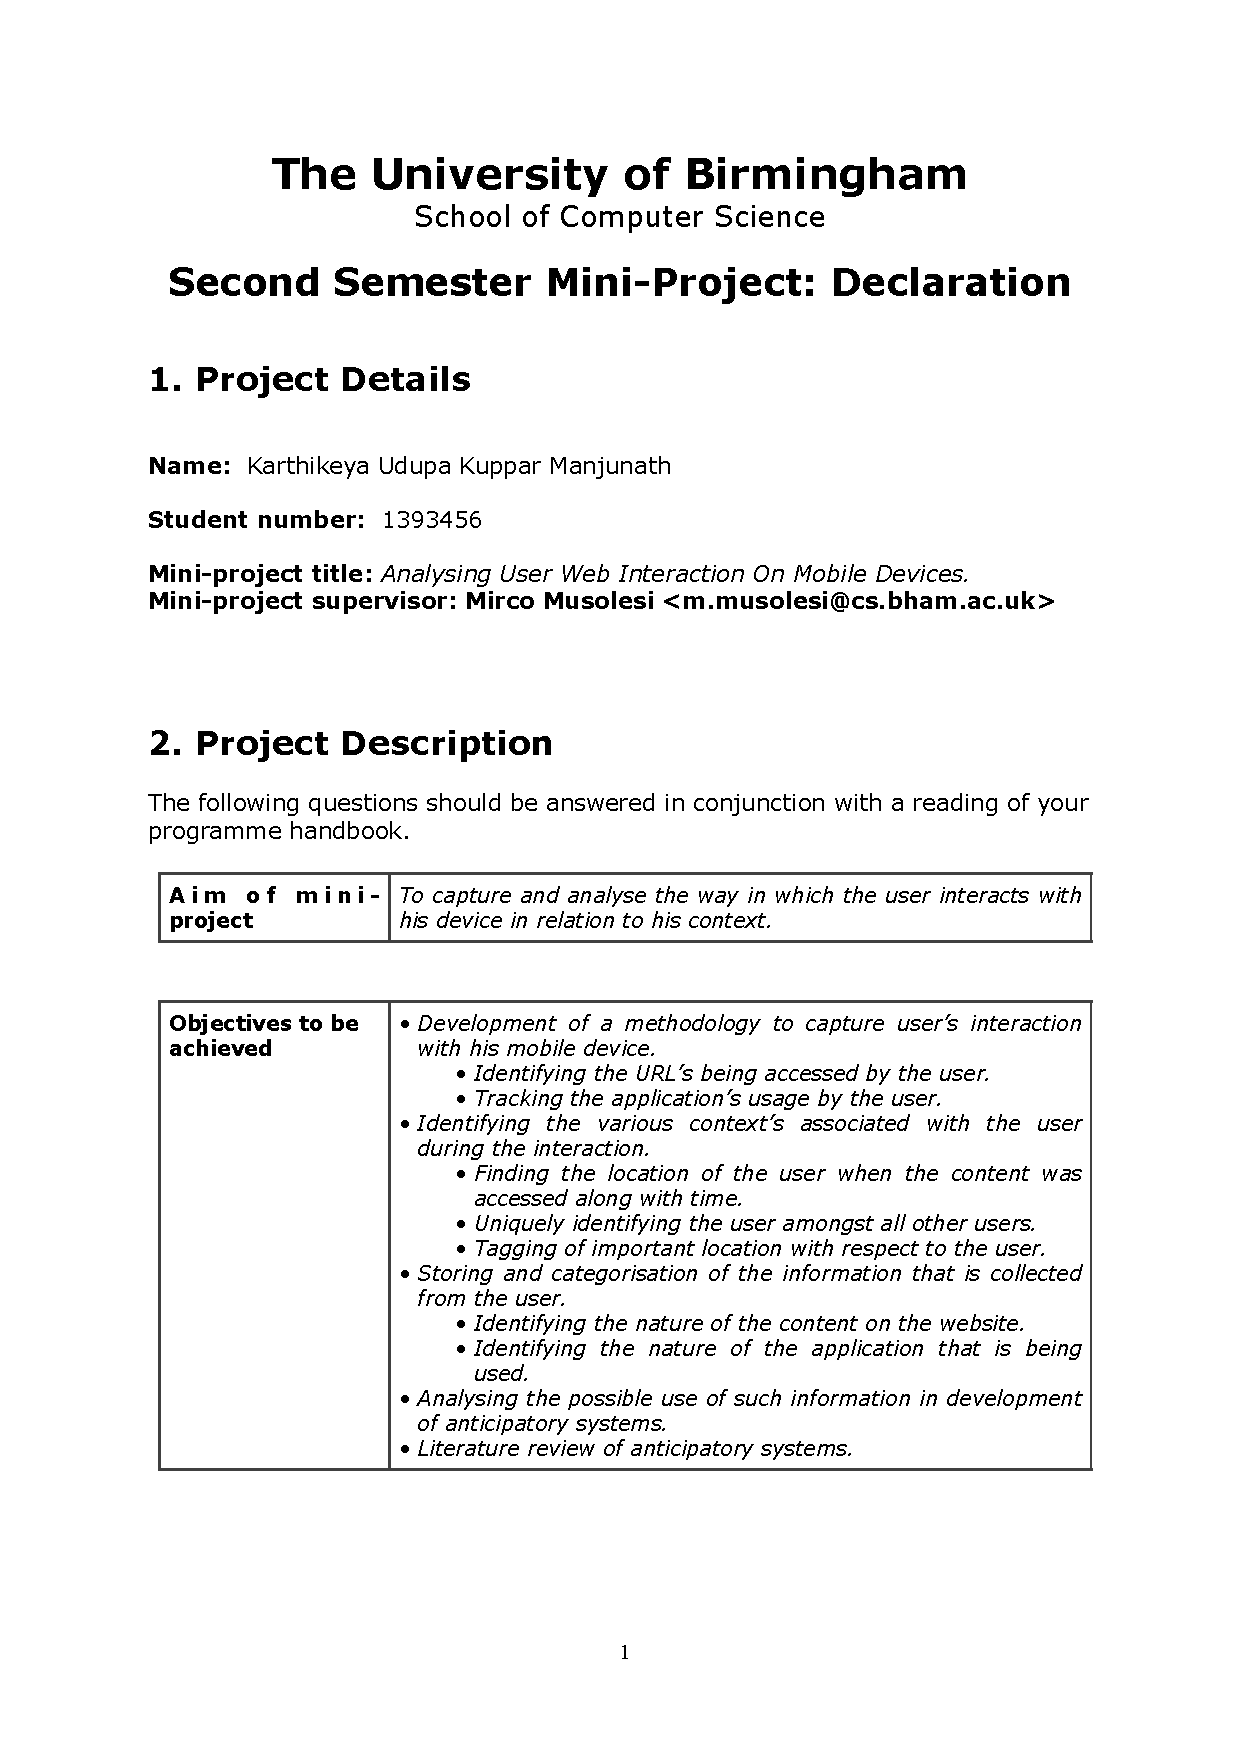
\includepdf[pages={1,2}]{Declaration.pdf}

\chapter{Statement of information search strategy}

statement of search
\end{document}